\chapter{Human Lumbar Vertebra Study} \label{Chapter_HT}

\section{Introduction}

Previous studies and the work in the earlier chapter have used a range of vertebrae, including
bovine, ovine and porcine among others. While all of these vertebrae have
important uses for developing methodology and understanding certain
characteristics, none share the trabecular structure, thickness of cortical
shell, axial strength or stiffness with human vertebrae. Hence, to understand the
mechanical effects of vertebroplasty in human lumbar vertebrae, human tissue is required.

Here, 14 lumbar vertebrae from four cadaveric spines have been used, with the
details shown in \cref{tab:vertebrae}. These spines were sourced from the Leeds GIFT 2 Research Tissue Project, with consent for the use of tissue being taken by the NHS Blood and Tissue Services.
These vertebrae underwent experimental
testing, augmentation, $\mu$CT scanning and the development of FE models
derived from their $\mu$CT scans. The goal of the chapter was to develop
methodologies to accurately model both augmented and non-augmented human lumbar
vertebrae. This chapter details the methods employed, the sensitivity tests
carried out, results acquired and a discussion of the implications of those
results.

\begin{table}[ht!]
\centering
  \caption{Details of the lumbar sections used from four cadaveric spines.}
  \label{tab:vertebrae}
  \begin{tabular}{c|c|c|c}
    Spine Name & Vertebrae & Sex & Age \\ \hline \hline
    Spine 1& L1, L2, L3, L4, L5 & F & 90\\ \hline
    Spine 2& L1 & F & 94\\ \hline
    Spine 3& L1, L2, L3 & M & 86\\ \hline
    Spine 4& L1, L2, L3, L4, L5 & M & 83\\ \hline

  \end{tabular}

\end{table}


\section{Experimental Methods}

This section describes the experimental methods used and developed to test and
record details of the set of human lumbar vertebrae. This includes an overview
of the major changes compared to the methods presented in \cref{chap_bov}, the
specifics of some of the new additions to these methods and the reasons for and
results of these improvements.


\subsection{Dissection \& Potting}

Th first step in the experimental setup, as with the bovine tail vertebrae, is
the dissection and potting of the vertebrae. As before, potting is required to
ensure parallel endcaps to allow repeated axial loading on materials testing
machines and dissection was required to remove the soft tissue that would
change the results given that only the bone is being tested and modelled.
Dissection of the human vertebrae gave added challenge compared to dissecting
the bovine tail vertebrae due to the degenerated nature of the vertebrae, with
fused facet joints common and difficulties circumventing the bone growths on
some of the most degenerated vertebrae.

The geometry of human lumbar vertebrae varies considerably to that of the
bovine
tail vertebrae from which this methodology is based. This is characterised by
much larger posterior elements with the facets extending much lower, below the
bottom of the vertebral body. Hence, to correctly pot the human vertebrae much
more cement must be used, especially for the posterior end-cap, to
cover the bottom of the vertebral body and the extending posterior elements.
This would lead to much more of the posterior elements being constrained, therefore
restricting the rotation of the vertebral body endplates under axial load. In
addition to this the larger posterior elements which are captured within the
PMMA end-caps will transmit load and take a greater share of the load when
compared to the bovine tail vertebrae. Given that vertebroplasty attempts to
restore the stiffness of the vertebral body and that there is no understanding
of specifically how the loads are shared between the vertebral body and
posterior element, this presents a problem.

A solution to this is to remove the posterior elements, following such methods
as \cite{Wijayathunga2008,RobsonBrown2014}, where only the vertebral body is
modelled. This allows the stiffness of the vertebral body alone to be captured
and modelled. The posterior elements were removed by cutting through the
pedicles at the narrowest part, limiting damage to the region.

To pot the specimens that now lack a spinal canal (which was used to aid
potting the bovine tail vertebrae), a retort stand was used to
hold the vertebra, ensuring that both endplates were level on average, given
that lumbar vertebrae do not have parallel endplates. %TODO illustrate?
The
specimen was then lowered down into the potting container leaving 5 mm between
the bottom of the vertebra and the container. PMMA was poured into the
container
until the entire of the endplate was touching cement, with the edges of the
vertebral body covered. Care needed to be taken to ensure all of the endplate
was in contact with cement, given the extent of osteophytes creating non-flat
surfaces in some of the more degenerated specimens. The other side of the
vertebra was potted in a similar manner, however, due to the constraints of the
potting container a measured quantity of cement was poured prior to lowering
the
vertebra into it. A spirit level ensured parallel end-caps.

\subsection{Loading}

Following previous studies \cite{Wijayathunga2008,furtado2007biomechanical}, the vertebrae were loaded
with an initial conservative maximum load of 800 N for similarly osteoporotic
vertebrae, rather than the high loads used by Pneumaticos et al.
\cite{pneumaticos2013effect}.
However, after loading two of the initial set of vertebrae the stiffness
continued to increase up to maximum 800 N. Following loads up to 2000 N showed
that the stiffness reached a maximum between 1300 and 2000 N, with three of the
initial four specimens showing some degree of failure in the final 400 N of
loading. Due to this failure, a maximum load of 1600 N was used as a compromise
for the remaining vertebrae used, although as presented below, some failure was
still observed.

\subsubsection{Maximum Stiffness Measurement}

The maximum stiffness of the vertebra was found in the same fashion as with the
bovine tail vertebrae - measuring the stiffness of segments at increments over
the length of the curve. Given that damage, especially for the intact
specimens,
needs to be avoided if possible the maximum loads used are on the conservative side. This
can mean that the maximum stiffness is potentially at the end of the data set
or
that the stiffness is still increasing at the load cut off. The solution to the
latter would require a prediction of the yield point prior to experimental
loading, while the former could
potentially be solved by using smaller segment sizes when measuring the
stiffness from load - displacement results.

To investigate the effect of segment size (the length of each section from which the
stiffness is found) and increment size (the size of each increment defining the
start point of each segment), the maximum stiffness finding Matlab script used
in the previous chapter was
rewritten in Python. This function could then be iterated over, reporting the
maximum stiffness when using an increment size of between 1 and 100 data points
(the distance between two data points corresponds to 0.0017 mm).


\begin{figure}[ht!]
  \centering
 
\includegraphics[width=6in]{Chapters/Chapter_HT_images/findStiffness_1incr.png}

 \caption{The effect of reducing the segment size on the maximum stiffness
    reported from four human vertebrae loaded to 2000 N pre and post
    augmentation. Using an increment size of 1 data point (0.0017 mm) and
    segment sizes of 100 to 1 data point (0.17 mm to 0.0017 mm).}
  \label{fig:findStiffness_1incr}
\end{figure}

\begin{figure}[ht!]
  \centering
 
\includegraphics[width=6in]{Chapters/Chapter_HT_images/findStiffness_20incr.png}
  \caption{The effect of reducing the segment size on the maximum stiffness
    reported from four human vertebrae loaded to 2000 N pre and post
    augmentation. Using an increment size of 20 data points (0.0037 mm) and
    segment sizes of 100 to 1 data point (0.17 mm to 0.0017 mm).}
  \label{fig:findStiffness_20incr}
\end{figure}

Using an increment size of one data point width, as shown in
\cref{fig:findStiffness_1incr} shows a smaller variation across the range of
segment sizes compared to using 20 points in \cref{fig:findStiffness_20incr}.
The effect of both segment size and increment
size is especially evident for the two Spine 2 L1 vertebrae both intact and
post
augmentation where the stiffness continues to increase until the end of the
test
at 2000 N. Meaning that there is a much smaller linear region for these two
specimens and hence a smaller segment size was required to measure the largest
gradient.

Choosing values for the segment size to use in the remainder of this study becomes difficult
given the large effect it can have on the measured maximum stiffness (a range
of
over 1000 N/mm in the case the two Spine 2 L1 tests). The segment size needs to
be small enough to capture the maximum stiffness while avoiding the noise (seen
to the right in \cref{fig:findStiffness_1incr,fig:findStiffness_20incr}) when
using a segment size below 18 data points. Hence, a value of 20 data points was
chosen, a value that avoids the noise while being on the plateau of the lines.


\subsubsection{Repeated Loading}

Given the nature of the test (attempting to limit damage to the vertebrae
especially during their initial non-augmented load), the ability to derive errors
becomes difficult especially from a single load. To attempt to understand this
error four vertebrae having undergone augmentation were tested three more times
in an iterative fashion, removing each from the load testing machine, testing
the next specimen in the set and repeating. Removing the vertebrae from their
steel housing (instead of three tests while seated in the steel housing)
allowed error in loading position and setup to be tested along with repeated
loading of the vertebrae.

The results of repeated loading can be seen in \cref{fig:exp_repeats}. The
majority of specimens show a reduced stiffness for the repeated loads following the
initial load, for which there are a few possible reasons. One possibility for
the reduction in stiffness is that it is a consequence of the freeze thaw cycle
that occurred between these tests. It could be
due to damage being caused during the initial load to 2000 N, in
\cref{fig:allLD} it is possible to see slight failure
in the three Spine 3 vertebrae, although failure cannot be seen in the Spine 2
L1 vertebrae, which also exhibits a reduction in stiffness in the repeats. An
option that may explain why for many of the vertebrae the change in stiffness
for the first repeat with different trends for the following two repeats is
that the vertebrae were seated differently in their endcaps for the first
repeat, settling into position for repeats 2 and 3. This trend of a different
stiffness for repeat 1 compared to 2 and 3 is evident in spine 1 L3 and L4,
spine 2 L1 and spine 4 L1, L2 and L3. A potential cause is the changing
temperatures (frozen to room temperature to above room temperature during the
$\mu$CT scan) causing the vertebrae to expand out of the endcap in some cases,
given the scan $\rightarrow$ freeze $\rightarrow$ back to room temperature
process used for the repeated loads presented.

The iterative reduction in stiffness for the Spine 3 L2 vertebrae can be
explained as damage being caused after each iteration. This can be seen in
\cref{fig:Spine3_L2}, with the three repeats each showing a yielding
before the 1600 N limit and a smaller maximum load and stiffness after each
repeat.

The figures in \cref{fig:allLD,fig:Spine3_L2} show the data for the
loading, from which the maximum stiffness values are found. This excludes the
initial cyclic loading, starts the loading at 50 N and displacement at 0 mm.

\begin{figure}[ht!]
  \centering
 
\includegraphics[width=\textwidth]{Chapters/Chapter_HT_images/experimental_repeats.png}
  \caption{The stiffness of the augmented vertebral specimens over the course
    of an initial load and three repeated loads.}
  \label{fig:exp_repeats}
\end{figure}


\begin{figure}[ht!]
  \centering
  \includegraphics[width=\textwidth]{Chapters/Chapter_HT_images/All_int_LD.png}
  \caption{The load - displacement results for the initial load for all used vertebra}
  \label{fig:allLD}
\end{figure}

\begin{figure}[ht!]
  \centering
  \includegraphics[width=\textwidth]{Chapters/Chapter_HT_images/spine3L2allrep.png}
  \caption{The load - displacement results for the Spine 3 L2 vertebra. Showing
    results of the intact load and post augmentation load as well as the 6
    repeats.}
  \label{fig:Spine3_L2}
\end{figure}





\subsection{Vertebroplasty}




Despite the development of methods for the augmentation of bovine tail
vertebrae, the methods for augmenting human vertebrae were altered due to the
different geometry, size and reduced density. 

The first change to the procedure was that the human vertebrae, being much less dense, did
not require the vertebroplasty needle to be inserted with the aid of a mallet.
Instead the needle could be pushed by hand through the cortical shell and into
the vertebral body, with the vertebrae being held in a vice to ensure the
correct angle and depth was achieved.

A second difference was the approach with the needle, instead of entering
the vertebrae through their pedicles an oblique approach was adopted. This was
due to variation in pedicle diameter between the L1 - L5 lumbar levels, where
the pedicles on the L1 vertebrae were very small and
therefore there was potential to damage the region and its load sharing capabilities.
The oblique approach therefore avoided damaging
pedicle-canal
region, especially for the L1 and L2 vertebrae with narrower pedicles.
An illustration of this approach can be seen in \cref{fig:vp-ill} with an
example $\mu$CT scan shown in \cref{fig:vp-ill_scan}.


\begin{figure}[h!]
  \centering
  \includegraphics[width=3in]{Chapters/Chapter_HT_images/vp_illustration.png}
  \caption{An illustration showing the approach to needle insertion and cement
position.}
  \label{fig:vp-ill}
\end{figure}


\begin{figure}[h!]
  \centering
 
\includegraphics[width=4in]{Chapters/Chapter_HT_images/vp_illustration_scan.png}
  \caption{A $\mu$CT scan showing the injected volume of cement at the anterior
of the vertebral body with the cement track from the exiting needle to the
right. For this specimen cement leaked through the anterior wall, limiting the
quantity of cement injected.}
  \label{fig:vp-ill_scan}
\end{figure}

A final difference to the needle insertion methods was a change to the needle.
Here, a side opening needle was used, allowing the cement to be directed into
the anterior-centre region of the vertebral body as opposed to directly out of
the needle end. This meant that larger cement volumes were much more achievable
given that the injection of cement was not aimed at the anterior wall and
instead could be rotated aiming both to the inferior and superior. One
limitation that this caused was increased difficulty backfilling the needle
tracks when the needle was removed. Future work may utilise a second
end-opening needle to perform the backfilling, in this case however there was
not enough time to change needles before the cement set, along with the
available needles having different gauges.

It was attempted to inject the largest possible volumes of cement into the
vertebrae, mimicking the clinical process.
Like the clinical procedure the injection was stopped upon cement leakage,
which generally occurred through one of the vascular channels at either the
posterior or anterior portions of the vertebrae.
However, despite stopping the injection upon cement leakage through vascular
channels, cement loss still occurred after the injection was stopped due to
pressure build up.
In addition to this, cement was also lost in the needle itself, where as the
cement set the amount of cement remaining in the needle became difficult to
measure.
This meant that the cement fill could not be accurately measured though the amount of PMMA
leaving the syringe due to both leakage and needle losses.
Hence cement fill volume was measured using segmented $\mu$CT scans, using the
volumes of the masks created to define the injected cement regions. This
methodology is described in the computational modelling section
(\cref{sec:comp_mod}).

\subsection{Vertebrae Characteristics}

Identifying the different characteristics for the set of lumbar vertebrae has
importance in understanding trends and relationships between the experimental
and computational results. For example a larger degree of anisotropy and hence
more directional and aligned trabeculae would potentially give a more
experimentally stiff vertebra, despite otherwise similar characteristics. Given
that much of the vertebral characteristics depend on the trabecular structure
it
is important to understand how this varies between specimens. Furthermore, any
calculations originating from a description of the trabecular structure require
a correct threshold to be applied to the $\mu$CT scan. This threshold describes
the limit of the trabecular bone and the start of either marrow or empty
space. To enable a fair comparison between vertebrae a region of interest was
selected from the vertebral body. Given the large variation in cortical shell
thickness, along with certain vertebrae containing large osteophytes and other
extra bone growth, the region of interest (ROI) was selected to be the largest
cylinder that could fit within the vertebral body while not capturing any of
the
cortical shell. %TODO add image of above (mebs?)

\subsubsection{Histograms}

In order to understand the spread of brightness' from the set of lumbar the
histograms of the ROIs were plotted (\cref{fig:normalisedhistogram}).

\begin{figure}[ht!]
  \centering
 
\includegraphics[width=4in]{Chapters/Chapter_HT_images/Normalised_Histogram.png}
  \caption{The normalised (with respect to the volume of the ROI) histogram
data
    for the 14 lumbar vertebrae.}
  \label{fig:normalisedhistogram}
\end{figure}

The lower greyscale values represent the empty space within the ROI which
translates to regions where the bone marrow has drained from the trabecular
bone, most likely
during the unavoidable freeze thaw cycles. The peak in the histogram at an approximate
greyscale value of 16 is due to the bone marrow. The remaining portion of the
histogram represents bone, where variation is due to the differences in the
mineral content of the bone, with more mineralised bone appearing brighter on
$\mu$CT scans. The specimens ROIs that contain the brighter values are those
that exhibit more degeneration for example Spine 2 L1, where the histogram is
shifted to the right, suggesting many more bright pixels and therefore more
bone spurs and other degeneration. This is because the extra bone growths on
the degenerated vertebrae is formed of denser cortical shell material.

\subsubsection{Threshold Optimisation}\label{th_opt}

Threshold optimisation or choosing a threshold that defines the limits of the
trabecular bone in terms of greyscale values is necessary for various parts of
the methods, the first being determination of the bone volume fraction (BV/TV)
and secondly for some of the computational modelling methods employed.

The full resolution scan is imported into imageJ where the threshold
optimisation is carried out.
The BoneJ plugin for imageJ is used for all of the trabecular structure
metrics, with the optimise threshold tool being the focus here.
The threshold optimisation feature works by optimising the connectivity
(Conn.D) against threshold value \autocite{Doubea2010}.
This tool is run on the region of interest using the default settings for the
connectivity options seen in \cref{tab:bonej}.
This chooses a threshold based on the peak in a connectivity against threshold
plot and reports that value.
These values can be seen in \cref{tab:optTH}, showing some variation across the
range of vertebrae.
However, the differences in these suggested thresholds can grouped with the
spine, for example: Spine 1 has a range between 15 to 17, while Spine 4 has a
range between 18 to 20.
This promotes the idea that these differences are due to the bone
mineralisation of the bone, especially given that the G17 spine is from a
Female and G41 from a male.

However, given that the chosen value for the threshold will directly impact the
reported metrics, a consistent value was chosen of 18. Using lower or higher
values for the threshold usually results in the trabeculae being described as
thicker or thinner respectively.
With respect to modelling, the difference in the mineralisation between specimens will still be
captured when using a fixed threshold, given that the binary image will be down
sampled before material properties are acquired. Here, thicker binarised
trabeculae correspond to a brighter continuum level voxel.
The results in \cref{tab:bv_tv_anis} show the BV / TV data and degree of
anisotropy values for the 14 specimens using the fixed threshold of 18.
Similar trends to what could be seen from the optimise threshold results can be
seen in the BV/TV data, with grouping between the
spines evident. This suggests that despite the use of uniform thresholds used
across the set of vertebrae the differences are still kept, giving some
additional validation and justification for using the uniform threshold.
The vertebrae from Spine 1 have a much lower bone volume fraction compared to the other
spines, which suggests a more osteoporotic spine, most likely resulting in less
stiff vertebra. The remaining discussion of these results is in
\cref{sec:exp_disc}.

\begin{table}[ht!]
	\caption{Settings used for the ImageJ plugin, BoneJ: Optimise Threshold.}
	\label{tab:bonej}
	\centering
	\begin{tabular}{c|c}
    Options & Values \\
    \hline
    \hline
    Tests & 11  \\
    Range & 0.2 \\
    Subvolume Size & 256 \\
    Erosian Cycles & 0 \\
    Dilation Cycles & 0 \\
    \hline
	\end{tabular}
\end{table}

\begin{table}[ht!]
	\caption{The suggested threshold from the optimise threshold BoneJ tool for
the 14 lumbar vertebrae in the set.}
	\label{tab:optTH}
	\centering
	\begin{tabular}{c|c}
    Specimen    & Suggested Threshold   \\ \hline \hline
    Spine 1 L1 & 17 \\
    Spine 1 L2 & 16\\
    Spine 1 L3 & 16\\
    Spine 1 L4 & 15\\
    Spine 1 L5 & 16\\
    Spine 2 L1 & 23\\
    Spine 3 L1 & 18\\
    Spine 3 L2 & 19\\
    Spine 3 L3 & 19\\
    Spine 4 L1 & 20\\
    Spine 4 L2 & 19\\
    Spine 4 L3 & 18\\
    Spine 4 L4 & 19\\
    Spine 4 L5 & 18\\
    \hline
	\end{tabular}
\end{table}



\section{Computational Methods}\label{sec:comp_mod}

The methods described in this section describe the process used to model
non-augmented and augmented vertebrae, with associated sensitivity tests to
understand the most appropriate approach to various aspects of the modelling
process.


The methods used in this section broadly follow those used in the previous
chapter, with a general process including the segmentation and FE model
generation in Simpleware ScanIP, and solving the models in Abaqus using setup
scripts written in python. One difference in this chapter is that the models
were run on ARC2, part of the High Performance Computing facilities at the
University of Leeds. Here, the submission of jobs (simple shell scripts
describing the process to be carried out) onto the cluster is carried out using
the Sun Grid
Engine, a first come first served scheduler for the cluster. By running the FE
simulation on the HPC cluster with resources: 10 cores, 1024 MB of memory per
core, the time to solve each model was reduced to 5 - 10 minutes compared to 20
- 40 minutes on a desktop PC depending on the model and material properties
used with models that included plasticity taking considerably longer to solve.
In addition to the time saving benifits this allowed off loading of large (5 -
10 GB per model) Abaqus output files and through the submission system it
allowed the iterative testing of material properties, where models could be
re-solved using different material properties read from a simple text file.

The methodology of using ARC2, one of the HPC clusters remained much the same
as when using a desktop PC. Here, abaqus input files were copied over to a user
directory on one of the cluster nodes, along with files detailing the loading
positions for the vertebrae, three python scripts and a shell script. The first
python script set up the model, importing each abaqus input file, applying
boundary conditions, loading position (according to the load position csv
file), creation of the  loading platen and application of the material
properties to the greyscale based material properties of the bone. Settings and
values applied in the setup script are read from another file containing: the
conversion factor (greyscale to Young's modulus), the displacement and for the augmented models the cement and
interface region material properties. The second python script runs the models
with values of the number of cores and memory to use matching those of the
requested HPC resources. The models are run with an initial increment of 0.1, a
minimum increment of 0.0001 and a maximum increment of 1. The final python
script runs the post processing; the abaqus output file is read and the axial
reaction force ($RF3$) is recorded. The resulting stiffness (reaction force divided by the
displacement to give a stiffness) from each model was written to a results file
which could be copied to the desktop PC and analysed. Finally, the shell script
describes the resources to be requested from the HPC cluster including a
maximum amount of time and then gives the command to be run: \texttt{abaqus cae
nogui=setup.py \&\& abaqus cae nogui=run.py \&\& abaqus cae nogui=post.py} for
the three python scripts. For new tests with potentially unexpected outcomes the abaqus output files were copied
to the desktop PC to be viewed, while if incremental material property changes
were being made, then only the stiffness results were copied.


\subsection{Non-augmented Vertebrae Modelling Using the BV/TV Method}\label{sec:non_aug_sens}

The methods used here broadly follow those described in the previous chapter with segmentation and model generation carried out in Simpleware scanIP and model simulation carried out in abaqus. Compared here in this chapter are two methods for modelling the non-augmented vertebrae, the first being named the normal method, which follows a near identical procedure to that used to model non-augmented bovine tail vertebrae. The comparison is made to a new method named the bone volume fraction, or BV/TV method. In this section the difference between these modelling methods are outlined with the bone volume fraction method being described in detail.

Given the aims of the project - to include the models generated here into a
larger set of vertebral models for use in statistical shape modelling, it is
useful to model the vertebrae in a scanner independent method. A method for
doing this (BV/TV modelling method) uses a full resolution scan with the bone
regions segmented and binarised using a threshold. This full resolution segmented scan is
then
downsampled to voxels with edge length of 1 mm, meaning that each voxel has a
greyscale value proportional to the BV/TV value for the region captured by that
voxel. Areas that contain more bone will therefore have a higher greyscale
value. This method is purely dependant on the threshold selected to define the
bone and hence, given that threshold values can be repeatedly and correctly
selected with the methods shown in Section~\ref{th_opt} through comparisons using phantoms, it can be scanner independent.



This method gives the opportunity to keep much of the detail that is often lost
when downsampling image data.  Specifically, the method described gives the
vertebral models much more definition of the cortical shell and internal
trabecular structure while maintaining the 1 mm cubed resolution and the
computational cost benefits associated.  The method follows similarly to the method used by Robson Brown et al.  \cite{RobsonBrown2014} with a few
minor changes. The scans are converted from the ScanCo proprietary ISQ format
into a stack of TIFF files using an in house Matlab script, which in
additionally reduces reduces the 16 bit data to 8 bit images.

The BV/TV method was compared to the normal method, described in \cref{finite-element-modelling-methods}, to understand the effect of the changes made and the use of different greyscale backgrounds.  For the bone
volume fraction method a threshold was applied at the full 82 $\mu$m
resolution.  This threshold was chosen to be a greyscale value of 18, the mean
of the values described in section Section~\ref{th_opt} and was applied to the
scan stacks in imageJ.  Once the binary stack was created a Gaussian filter was
applied, also within imageJ, with $ \sigma_{x,y,z} = 1 $.  This was applied in
order to remove speckling found surrounding the end-caps and some of the other
noise visible in the scans.  The two stacks of images, binary and non-binary, are then imported into
ScanIP; carried out by opening one stack of images (the original stack) and
then importing a second background (the binary image stack). Both backgrounds
are downsampled to voxel sizes of 1 mm$^3$, with the (originally) binary stack
being used to create the mask for the vertebrae and the original stack being
used for the segmentation of the end-caps.  Greyscale material properties for the vertebral mask
are taken from the binary stack, while the remainder of the methods follow the
same process as the original method.  A comparison of the two approaches can be
seen in \cref{fig:normal_vs_bv_tv_seg}, where the improved definition of
trabecular structure and cortical shell using the bone volume fraction method
can be seen in E and F, following the downsample to 1 mm$^3$ resolution.

\begin{figure}[ht!]
\centering
\includegraphics[width=.65\textwidth]{Chapters/Chapter_HT_images/normal_vs_bvtv_seg.png}
	\caption{A comparison of the normal method (A, B and C) and the bone volume
fraction method (D, E and F). A shows the full (82 $\mu$m) resolution scan, B
shows the same image downsampled to 1 mm resolution and C shows the segmented
scan. D shows the segmented bone at 82 $\mu$m, E shows this image downsampled
to 1 mm and F shows this image after segmentation.}
\label{fig:normal_vs_bv_tv_seg}
\end{figure}

%\begin{figure}[ht!]
%  \centering
% \includegraphics[width=6in]{Chapters/Chapter_HT_images/diffModellingMethods.png}
%  \caption{The stiffness results of three different FE methods for four intact
%    human vertebrae compared to the experimental stiffness results. Interest
%    should be drawn to the ratio between specimen models rather than thevalues
%    themselves, given that the conversion factors between greyscale values and
%    Young's modulus have not been optimised at this stage. Results show the
%    difference between the currently used method of modelling the vertebraeand
%    the BV/TV based methods (both with uniform thresholds and different
%    thresholds for each specimen).}
%  \label{fig:diffModellingMethods}
%\end{figure}




%\subsubsection{Predicting Vertebral Yield Point}\label{predYield}

\subsection{Sensitivity Studies}

Sensitivity studies other than the main BV/TV tests present difficulties due to the models reliance on
the underlying greyscale background.  This is due to the greyscale optimisation
process required to obtain a new conversion factor between the greyscale values
and the Young's modulus for every change made to the material properties or
boundary conditions of the models.  This is in order to understand the effect
the change has on the agreement between experimental and computational results,
and because a change to the material properties or boundary conditions may not
have a systematic or uniform effect on the results.  Due to this, simple
sensitivity tests become difficult, including common convergence studies on voxel size. The sensitivity studies in this section highlight tests that were carried out that either did not require re-calibration of the greyscale conversion factor, or had minimal re-calibrations.

\subsubsection{Load Position Sensitivity}

With a dual aim of understanding the error in choosing the load position for the model (aiming to match the experimental loading point as closely as possible) and to  understand how the vertebrae respond to different loading
positions, 16 different positions were tested, shown in
\cref{fig:loading_pos}.
These positions included 1~mm and 2~mm aways from the centre in the posterior,
anterior, left and right directions along with larger deviations of 10~mm and
20~mm from the centre in the same directions.
The same boundary conditions, along with the 1 mm of axial displacement described
above were applied to the different loading positions and the change in
stiffness was recorded. The two magnitudes of distances from the centre tested, 1 and 2 mm, and 10 and 20 mm, are used to test the error due to the 1 mm resolution and the understand the response to non-central loading respectively.

\begin{figure}[ht!]
\centering
\includegraphics[width=.7\textwidth]{Chapters/Chapter_HT_images/Loading_positions_Human.png}
\caption{The loading positions used for the load variation tests. Position X is
the original central loading position for ap and lr loading, other loading
positions are 1~mm, 2~mm, 10~mm and 20~mm away from the centre.}
\label{fig:loading_pos}
\end{figure}


The results of the load position sensitivity tests (\cref{fig:hum_load_ap})
show that on average, small posterior loads (above denser bone) result in
higher stiffness's while all anterior loads result in a reduced stiffness.
Loads lateral to the central loading point (\cref{fig:hum_load_lr}) resulted in
little mean change to the stiffness of the models for the 1 and 2~mm
positions.
Larger movements away from the central loading position (10~mm and 20~mm)
result in almost all vertebrae presenting a reduction in stiffness.
Loading positions at 20~mm left and right present the largest reductions, where
in the natural body the expected loads are less compared to anterior/posterior
loading.
Additionally, larger anterior loads resulted in larger reductions in the
stiffness, given the less dense nature of anterior portions of the vertebral
body

It also shows that the effect of movements of 1 mm away from the experimental
loading position only changes the stiffness by approximately 5 \%.
Given the resolution of the models is limited to 1 mm, the accuracy of the
selection of the experimental loading positions is also limited to 1 mm.
The maximum 5 \% change to the stiffness when posterior or anterior may
describe some of the error seen when comparing the experimental and
computational results. However, as discussed in more detail in \cref{sec:errors}, these errors may be negligible compared to the errors in the acquisition of the experimental stiffness from load-displacement data.

\begin{figure}[ht!]
\centering
\includegraphics[width=\textwidth]{Chapters/Chapter_HT_images/hum_ap.png}
\caption{The effect of the loading position for the human lumbar vertebrae,
shown as a percentage change compared to a central loading position, for load
positions from the posterior to anterior according to \cref{fig:loading_pos}}
\label{fig:hum_load_ap}
\end{figure}

\begin{figure}[ht!]
\centering
\includegraphics[width=\textwidth]{Chapters/Chapter_HT_images/hum_lr.png}
\caption{The effect of the loading position for the human lumbar vertebrae,
shown as a percentage change compared to a central loading position, for load
positions from the left to the right according to \cref{fig:loading_pos}}
\label{fig:hum_load_lr}
\end{figure}



\subsubsection{End-cap Depth \& Contact sensitivity}
This sensitivity test was carried out due to the high regions of stress seen in when removing the endcaps from the scene in the abaqus output viewer.
The stress distribution at the surface of the vertebral body shows high stress
at the edges of the cement endcaps, at both the top and bottom of these
regions, shown in \cref{fig:stress_lines}.
Experimentally the endcaps are merely moulded to the shape of the top and
bottom of the vertebral body allowing slight motion of the vertebrae within them. However, previous work and other studies have
used tied contacts between the bone and endcaps, removing any motion between the
two and locking neighbouring nodes together.
Additionally, the depth of these endcaps varies between 5 mm and 20 mm
depending on the shape of the vertebral endplates.
The more concave the vertebral endcap was the more cement was required to fill
the space forming a flat cement surface. Hence, those models with larger endcaps may have more error given that more of the model was tied and therefore constrained within the endcaps. However, no relationship between cement endcap depth and the stiffness or error in the stiffness compared to the experimental result was found.

\begin{figure}[h!]
\centering
\includegraphics[width=.65\textwidth]{Chapters/Chapter_HT_images/stress_lines.pdf}
\caption{The effect of having tied contacts between the endcaps and the bone,
with the increases in Von Mices stress indicated.}
\label{fig:stress_lines}
\end{figure}


Given this variation, tests identifying the effect of changing the endcap depth
were carried out using FEA models with different depths of $\pm$ 1, $\pm$ 2 and
$\pm$ 3 mm for the top and bottom endcaps independently and together.
Additionally, the effect of changing the cement endcap depth with the currently used, tied contact to a frictionless
contact was also investigated, along with variations to the properties of the
frictionless contacts.

The endcap depth was altered by adding and removing layers within the model
file in ScanIP, re-meshing the model and running the files using the same
Abaqus python scripts.
Endcap contacts were changed within the Abaqus python scripts, by firstly
removing the ties between the endcap and the vertebra.
An interaction property was created with tangential behaviour set to
frictionless and normal behavior with properties: $pressureOverclosure=HARD, 
constraintEnforcementMethod=Default$ and the final option was experimented
with, $allowSeperation=ON/OFF$.
The $allowSeperation$ variable determines whether separation is permitted once
contact is established and initially models ran correctly with it set to its default of
$ON$.
However, when experimenting with the effect of loading position, especially
with loads applied far from the vertebral centre, the solver struggled to
converge due to the high stresses this caused at the limits of the vertebral body.
Disallowing separation after contact was shown to have a small effect on the
results (the outputted stiffness, with a mean increase in stiffness of 63 N) and allowed the models to run to the
completion of the job. 
The remaining settings were set to the default for a generic contact: 

$
	initialClearance=OMIT \\
	adjustMethod=None \\
	sliding=SMALL \\
	enforcement=NODE\_TO\_SURFACE \\
	thickness=ON \\
	supplementaryContact=SELECTIVE \\
	interactionProperty=contactName \\
	smooth=0.2 \\
	bondingSet=None \\
$

The results shown in \cref{fig:with,fig:without} show that regardless of the
contact, increasing the depth of the endcaps significantly increases the
stiffness of the vertebrae, while reducing the depth reduces the measured
stiffness.
The effect this extra or reduced constraint caused by the changing endcap depth
broadly follows the same trends for the two vertebrae tested.
However, the response does differ most notably at the extremes of endcap depths
($\pm$3 mm), where the spine 4 L5 vertebrae experiences the greater reduction
in stiffness when reducing the endcap depth, while the spine 1 L2 vertebrae
sees the greater increase following depth increases.
This difference is a consequence of the differences in the density of the
vertebrae (where spine 4 is, on average, much denser than spine 1 in terms of
mean greyscale value) and the differences in the shape (the L5 vertebrae being
much wider with greater protruding bone spurs at the bottom of the vertebrae
and the narrower L2 vertebrae having the bone spurs at the top of the
vertebrae.
These shape differences can be seen in \cref{fig:Spine 1_projection,fig:Spine
4_projection}.

The variation in the change to the stiffness within $\pm$ 1mm change in depth
was up to 5 \%, for both cases.
Given that the maximum error in masking the cement endcaps is 0.5 mm due to the
resolution that is used for the segmentation, it suggests that this error has a
minimal effect on the end results. As mentioned previously, this is due to the other errors associated with with measuring the experimental stiffness.

The effect of changing the contact from tied to frictionless can be seen by
comparing \cref{fig:with,fig:without}.
Excluding the very large change in stiffness seen in the L5 vertebra when
reducing the depth of the inferior endcap, the adoption of the frictionless
contact reduces the effect of endcap depth on
measured stiffness.
This is due to a reduction in the constraining nature of the frictionless
contact, allowing a more natural measure of the vertebral stiffness rather than a combination of the vertebral and endcap combined stiffness.
The anomalous L5 vertebrae here is a function of having less support and the
slipping that this allowed, resulting in the reduced measured stiffness.
Optimising the greyscale conversion factor for the set of models with a tied
constraint and a frictionless contact gave an improved agreement with a concordance correlation coefficients
of 0.848 and 0.865 respectively.
Therefore the frictionless contact providing a small improvement in the
agreement between the computational and experimental results.





\begin{figure}[h!]
\centering
\includegraphics[width=\textwidth]{Chapters/Chapter_HT_images/with.pdf}
\caption{The percentage change in stiffness following a change to the endcap
thickness. Inf and Sup show changes of $\pm$ 1, 2 and 3 mm to the inferior and
superior endcap depth respectively. The endcaps have a tied contact to the
vertebrae.}
\label{fig:with}
\end{figure}

\begin{figure}[h!]
\centering
\includegraphics[width=\textwidth]{Chapters/Chapter_HT_images/without.pdf}
\caption{The percentage change in stiffness following a change to the endcap
thickness. Inf and Sup show changes of $\pm$ 1, 2 and 3 mm to the inferior and
superior endcap depth respectively. The endcaps have a frictionless contact to
the vertebrae.}
\label{fig:without}
\end{figure}

Further tuning of the specifics of the frictionless contact could be carried
out (to see if an improved agreement could be achieved) and would be a simple
addition to this sensitivity test.
However, due to the greyscale conversion factor optimisation process required
to test each option this would be a timely operation, which, given the relatively small
effect of changing to the frictionless contact, could yield negligible
results.




\subsection{Material Properties}

The general method for obtaining material properties for the bone elements in the
FE models uses the same approach as used in \cref{material-properties-bov}
where the Young's modulus of each element is equal to the greyscale value
multiplied by a conversion factor.
The conversion factor is optimised by comparing the computational stiffness
against the experimentally acquired stiffness.
For the optimisation process the vertebrae were split into two groups at
random, giving a calibration and validation set, allowing a test of the
validity of the greyscale conversion factor.
The split of the vertebrae for these two sets can be seen in
\cref{tab:calib_valid}, where the greyscale conversion factor was derived from the calibration set and applied to the validation set where the agreement was measured.

\begin{table}[ht!]
	\caption{The vertebrae used for the calibration set and the validation set in
the optimisation process.}
	\label{tab:calib_valid}
	\centering
	\begin{tabular}{c|c}
    Calibration Set   & Validation Set  \\ \hline \hline
    Spine 1 L4 & Spine 1 L1  \\
    Spine 1 L5 & Spine 1 L2\\
    Spine 2 L1 & Spine 1 L3 \\
    Spine 3 L2 & Spine 3 L1\\
    Spine 4 L1 & Spine 3 L3\\
    Spine 4 L2 & Spine 4 L3\\
    Spine 4 L4 & Spine 4 L5 \\
    \hline
	\end{tabular}
\end{table}


Results from the initial optimisation process using the calibration and
validation processes gave good results: the agreement of the validation
set had CCC values of above 0.5.
The validation set for the ``normal" method had a CCC value of 0.591 and the
CCC value for the validate set from the ``bone volume fraction" method gave a
value of 0.831.

Given the problems associated with calculating the greyscale conversion factor
with various sensitivity tests described in \cref{sec:non_aug_sens}, the
calibration and validation sets were only used for the initial test, once using
the ``normal" method and once using the ``bone volume fraction" method.
This validated the use of the optimisation process while allowing more accurate
greyscale conversion factors for the sensitivity tests and final values given
that the input set of human vertebrae was relatively small.


\subsection{Final Material Properties and Boundary Conditions for the Non-augmented Models} \label{sec:nonaugmatprop}

Following the results of the sensitivity tests the final value from the
optimisation process for the greyscale conversion factor was 0.0009625 for the BV/TV method and 
This was used for the bone properties for all final non-augmented models and
augmented models. The optimised greyscale conversion factor for the models generated using the normal method used a value of 0.00416.

The remaining material properties used for all of the models are a Poisson's
ration of 0.3 for the bone and endcaps and a Young's modulus of 2.45~GPa for
the endcaps. Boundary conditions for the models included the frictionless contact between the vertebrae and their endcaps (for the bv/tv method, tied for the normal method), a tied contact between the analytical platen and the superior endcap where 1 mm of axial load was applied. 



\subsection{Modelling Augmentation}

Given the limited validation of models achieved using bovine tail vertebrae
(due to the reasons discussed in Section~\ref{bov:results}), a range of
different material properties and approaches to modelling the bone-cement
interface were investigated.
In addition to varying the material properties of the injected volumes of
cement, the effect of using a combination of scans from before and after
augmentation has been experimented with.
To achieve this scans of pre/post augmentation were registered.
This method utilised the BV/TV method described earlier, where the
non-augmented full resolution binary scan is registered to the full
resolution augmented scan.

\subsubsection{Registration of $\mu$CT Scans}

Artificial brightening of regions surrounding the internal cement (specifically
the concentrated volumes of barium sulphate and the artefacts associated)
affect the material properties that are applied to the material, seen in the
right side image in \cref{fig:reg_demo}. Given that the material properties are based on the greyscale background, this has the effect of artificially stiffening or changing the properties of elements who's properties are described by these regions.
To bypass this effect the two models, intact and post-augmentation models can
be registered - translating them into the same spacial location.
This allows the cement to be defined, masked and modelled based on the
post-augmentation scan and the remaining vertebra to be defined from the non-augmented
scan, using same background used for the non-augmented models.
While the shape of the vertebra may have been changed over the course of its
two loads, this change is less than what can be seen at 1 mm resolution and is
not apparent during the registration process carried out at 82 $\mu$m
resolution.
%Additionally regions that have experienced damage through the insertion of the
%needle, yet do not contain cement, will also be neglected using this method.
%However, the same justification can be made, where this is unlikely to have any
%affect at 1 mm resolution.

Registration of the images was carried out in 3D Slicer, using scans of the
segmented, full-resolution, non-augmented vertebrae and the full-resolution
augmented vertebral scans.
The method of registration was a landmark based approach using three landmarks
for each vertebra, translating the scan of the augmented vertebrae to that of the non-augmented vertebra.
These points were selected at the most superior point of one pedicle, the most inferior point of the
other pedicle and the most inferior and anterior point of the vertebral body.
The selection of these points proved to provide a repeatable registration of
the vertebrae, without selecting superfluous landmarks.
Once registered the resulting translated augmented vertebrae scan was cropped
with respect to the non-augmented scan to provide an aligned and registered
pair of scans.

\begin{figure}[ht!]
  \centering
  \includegraphics[width=4in]{Chapters/Chapter_HT_images/reg_demo.png}
  \caption{An illustration of the registration process, registering the
non-augmented scan (left) with the augmented scan (right). The images are at 1
mm resolution, showing the artifacts created by the barium sulphate when viewed
at this resolution, while to increase accuracy the registration carried out in
Slicer 3D was at the full 82 $\mu$m resolution.}
  \label{fig:reg_demo}
\end{figure}

\subsubsection{Registered Scan Model Generation}

The augmented models using the registered scans were created in ScanIP,
following similar methods to the bone volume fraction method described in
Section~\ref{bvtv_method}.
The initial step was to import the registered augmented scans and apply an
initial downsample to a resolution of 0.5 mm$^3$.
This resolution provided enough detail to capture the detail of the injected
cement volume without increasing the computational difficulty and therefore
time to segment the scans.

To segment the three regions (background, bone and endcaps, and injected
cement) it was found that the most reproducible and accurate method was to use
the Otsu thresholding process \cite{sezgin2004survey}, a filter that is built
in to ScanIP\@.
It was used to find four masks in the scan and works on a threshold clustering
method.
In this case searching for four clusters or masks separated by different
thresholds and returning a mask that described the background, bone,
endcaps and the cement region.
From this only the cement mask was retained.
The mask and background were then downsampled to 1 mm resolution and cropped to
the same dimensions as the non-augmented model.
From the non-augmented model, the masks describing the vertebra and endcaps were imported, along with the binarised background of the vertebra.
The origin of the masks coming from the two backgrounds can be seen in
\cref{fig:mask_demo}.

\begin{figure}[ht!]
  \centering
  \includegraphics[width=4in]{Chapters/Chapter_HT_images/mask_demo.png}
  \caption{An illustration showing the origin of the masks from the
non-augmented scan (left) and the augmented scan (right).}
  \label{fig:mask_demo}
\end{figure}

Finally, given that the non-augmented $\mu$CT scan is used for the material
properties of the augmented models when using the method outlined above, damage
caused to the vertebrae during the augmentation process is not captured in the
model. Specifically the track left behind by the vertebroplasty needle is shown
clearly on the post-augmentation $\mu$CT scan, and while it was attempted to
fill this space when cement when removing the needle in some cases this was not
possible or the needle track was only partially filled. An example of the track
left behind can be seen in \cref{fig:needle_track}:B, with comparisons to the
BV/TV background in A, and the correction, through removal of the mask in C.
Removal of the vertebral mask in the regions where the needle track was clear
in the post-augmentation scan was carried out using the (un)paint line tool in
Simpleware ScanIP. This change to the models required further changes to the material
properties of the cement and interface regions as described in
\cref{sec:cemmatprop}. Results of models with and without the needle track are presented in \cref{sec:augcompres}.

\begin{figure}[ht!]
  \centering
  \includegraphics[width=4in]{Chapters/Chapter_HT_images/needle_track.png}
  \caption[Adding the needle track to registered models.]{Adding the needle
track to registered models. A, shows the masks
overlaid onto the BV/TV greyscale background, B shows the masks overlaid onto
the augmented scan background and C shows the removal of the mask where the
cement track is visible. The pink mask shows the cement region, yellow shows
the
interface and red is the vertebral mask.}
  \label{fig:needle_track}
\end{figure}

\subsubsection{Cement Volume Material Property Tests} \label{sec:cemmatprop}

Based on the results of the tests carried out on the bovine tail vertebrae in
\cref{chap_bov}, different material properties and approaches were attempted to
further the agreement between the experimental and computational results of
augmented vertebrae.  These were mainly changing the material properties of the
interface layer between the bone and the cement, along with the material
properties of the cement volume itself.

These material properties were tested in an iterative fashion changing the
properties in the material properties file read by the python setup script.
Following the results of the above tests, the final material properties for the
cement and interface regions are in \cref{tab:matprops4cmt} for the three main methods tested.

\begin{table}[h]
\centering
\caption{The material properties for the injected cement volumes and it's
	surrounding interface region for the three main modelling methods
used. P.P., indicates perfectly plastic}
\label{tab:matprops4cmt}
\begin{tabular}{c|c|c|c}
               & \multicolumn{3}{c}{Modelling Method}				\\
	\hline 
	Property	       & Non-registered & Registered & Registered  \\ 
			       &		&	     & With Needle
	Tracks \\ \hline \hline
Cement Young's Modulus    &1.7 GPa            & 1.2 GPa       & 1.5 GPa \\
Cement Poisson's Ratio    &0.4                & 0.4           &0.4  \\ \hline
Interface Young's Modulus & 0.005 GPa          & 0.008 GPa      &0.01 GPa \\ 
Interface Poisson's Ratio & 0.4               & 0.4           & 0.4\\ 
Interface Yield Stress	  & 50 Pa $\rightarrow$ P.P.      & 5 Pa $\rightarrow$
P.P.  & 5 Pa $\rightarrow$ P.P.
\\ \hline
\end{tabular}
\end{table}

Boundary conditions for the cement region include: tie contacts between the
vertebrae and interface, and between the interface and the cement volume.
The remaining material properties and boundary conditions remain the same as
with the non-augmented models, described in \cref{sec:nonaugmatprop}.

Finally, an alternate way of modelling the augmented region was attempted using
the greyscale background of the non-augmented specimen to serve as a measure of
the location of the cement. If the element was bright, suggesting it contained
mostly bone, it suggests that the element does not contain cement. Conversely
low greyscale value elements suggests limited bone and therefore more chance of
containing cement. However, the initial testing using this methodology produced
a poor agreement with the experimental results and investigation and
optimisation of the method was stopped. The methodology and limited results are
described in \cref{sec:invGS}.

\subsection{Measuring the Vertebral Body \& Augmentation Volume}
\label{sec:measure}
While the volume of the vertebral mask can be measured directly within ScanIP
or Abaqus, this volume includes the remainder of the pedicles and other bone growths and spurs.
The size of the pedicles that remain after their removal during dissection
varies between level and spine and is especially different with the level five
vertebra, where the shape and size varies dramatically.
To account for this variation and to get a more accurate cement fill percentage
for the augmented models elliptic cylinders were fitted to the vertebral body
as shown in \cref{fig:cyl_fit}.



\begin{figure}[ht!]
  \centering
 
\includegraphics[width=5in]{Chapters/Chapter_HT_images/cyl_fit_ful_iso_both.png}
  \caption{A diagram showing the fitting of the cylinders to the vertebral
body, where the point cloud describing the vertebra comes from an STL file, the
red ring shows the points included in the mid-slice and the central red dot
indicates the center of the mid-slice.}
  \label{fig:cyl_fit}
\end{figure}


This was carried out using a set of scripts written in python and rely of
having stl files describing the vertebral geometry.
The scripts work by finding the middle slice of a set of nodes that describe
the vertebra.
From the middle slice the shape of the ellipse is formed.
Given that the alignment of the vertebrae is uniform, the mid point on the $y$
axis is found by searching for the node furthest away from the weighted center,
$\pm$ 2 mm of the weighted centre. The axes are defined in \cref{fig:cyl_fit}:B.
This gives the $a$ measure of the ellipse description.
The $b$ measure is found by using a similar process - searching for the node
furthest away from the centre on the $x$ axis, within $\pm$ 2 mm.
The $a$ and $b$ measures gave the shape of the ellipse and the height of the
elliptic cylinder was found by raising and lowering the ellipse until a node in
the middle $\pm$ 5 mm of the endplate intersected the ellipse.
This defined the height of the ellipse.

Vertebrae that contained a vascular channel, seen in \cref{fig:cyl_channel},
had the channel removed by filling the space in ScanIP.
This was carried out for two main reasons: the first was to allow accurate
fitting of the cylinder into the vertebral (to avoid the problems shown in
\cref{fig:cyl_channel}) and to remove problems with the cement being exposed
when modelling augmentation and the extra contacts / interfaces that are
created.
Models with the vascular channel removed were compared to the original models
and it was found that there was less than 0.5 \% difference for the set.
This was due to the elements used to fill the channel having material
properties based on the greyscale, which had values of approximately zero,
given the nature of the channel.
Due to the lack of any effect in removing the channel the vertebra models of
augmentation did not include the vascular channel.

\begin{figure}[ht!]
  \centering
 
\includegraphics[width=5in]{Chapters/Chapter_HT_images/cyl_fit_channel_both2.png}
  \caption{An illustration showing the problems that occur with vertebrae that
have a distinctive vascular channel and the false cylinder fit that occurs.}
  \label{fig:cyl_channel}
\end{figure}


The volume of the ellipse was found (V = $\pi a b h$, where $a$ and $b$ have
been described and $h$ is the height) and compared to that of the total
vertebral volume, shown in \cref{tab:vertebrae_vol_cyl}.
The percentage reduction in vertebral body volume, from total vertebral body
volume to the fitted cylinder volume, varies significantly and is due to
changes to the vertebral shape outside of the main vertebral body portion.
For example, Spine 2 L1 was a degenerate vertebrae with extra bone growth at
the anterior limits of the vertebral body.
Other large changes were due to the size of the pedicles, where larger
vertebrae (Spine 4) had proportionally larger pedicles.

\begin{table}[ht!]
\centering
  \caption{Vertebral body volume compared to the volume of the fitted
cylinder.}
	\label{tab:vertebrae_vol_cyl}
  \begin{tabular}{c |c|c|c}
	  Specimen & Total Vertebral  & Fitted Cylinder & Change in Volume\\ 
	  &Body Volume (mm$^3$)&Volume (mm$^3$) &(\%)\\ \hline \hline
	  Spine 1\_L1  & 31229 & 17490 & -44\\
	  Spine 1\_L2  & 31789 & 20551 & -35\\
	  Spine 1\_L3  & 33519 & 22014 & -34\\
	  Spine 1\_L4  & 35123 & 22796 & -35\\
	  Spine 1\_L5  & 31189 & 22254 & -28\\
	  Spine 2\_L1  & 33835 & 17420 & -48\\
	  Spine 3\_L1  & 45866 & 31073 & -32\\
	  Spine 3\_L2  & 53695 & 34470 & -36\\
	  Spine 3\_L3  & 56003 & 36750 & -34\\
	  Spine 4\_L1  & 35137 & 22231 & -37\\
	  Spine 4\_L2  & 36791 & 23837 & -35\\
	  Spine 4\_L3  & 39909 & 26036 & -35\\
	  Spine 4\_L4  & 43357 & 25612 & -41\\
	  Spine 4\_L5  & 45606 & 26936 & -41\\
	  \hline
  \end{tabular}

\end{table}

The effect of this change on the relationship between cement fill and change in
augmentation stiffness was identified and is shown in
\cref{fig:cyl_fit_comparison}.
While there was a change in the relationship, a clear trend between the cement
fill percentage and change in stiffness for the majority of the vertebrae is
still not evident using wither approach to measuring the vertebral body volume.

\begin{figure}[ht!]
  \centering
 
\includegraphics[width=.7\textwidth]{Chapters/Chapter_HT_images/cyl_fit_comparison.png}
  \caption{The effect of using the fitted cylinder as a measure of vertebral
body volume, on the relationship between augmentation fill volume and change in
stiffness following augmentation. The red points show the relationship using
the total vertebral volume, with the relationship using the fitted cylinder
shown in blue.}
  \label{fig:cyl_fit_comparison}
\end{figure}


\subsection{Visualisation of Vertebrae and Augmentation}

\subsubsection{Vertebral Density Visualisation}

To visualise to the density distribution of the trabecular bone within the FE
models, Simpleware ScanIP was used. Here, FE models were generated and the clip
box was used to remove an axial half of the model from the render. Mass density
material properties were then assigned to the model within the visibility
options, given that material properties for the region had been set to
greyscale based. This provided color maps of the density of the vertebral
mid-slice. An example of this can be seen in \cref{fig:HT_gs_map}.

\subsubsection{Cement Distribution  Visualisation}

Visualisation of the cement distribution in augmented vertebrae can be
difficult due to the 3D nature of the cement distribution. Understanding features of the cement volume, for example determining
whether cement volumes are distributed or concentrated becomes difficult.
Given that 2D images of the augmented vertebrae only give an understanding of
the layer in question and the 1 mm resolution of FE
models makes identifying the nature of the structure from the generated model visualisation difficult.
The methodology used to visualise the vertebrae and the solution to this
problem was to use the 3D project feature in imageJ. This creates a 3D
rendering from the stack of images and rotates the resulting object through a
range of angles, in this case 360 degrees. Variables of transparency bounds,
opacity bounds and the projection method can be set, in addtion to the axis of
rotation. These were left at their default using the brightest point projection
method and the Y-axis for the rotation axis. This generated a model that could
be rotated arround the Y-axis, providing a view of the cement distribution
though the vertebrae and not one limitted to a slice by slice view. Examples of
this method can be seen in \cref{fig:Spine 1_projection,fig:Spine
2_projection,fig:Spine 3_projection,fig:Spine 4_projection}, where projections of the
transverse and saggital planes can be seen. 



\section{Results}

The results described in this section are split into two main sections: those derived and obtained through experimental means and those measured from the computational, generated models.

\subsection{Experimental Results}\label{sec:aug_stiffness_res}

Material properties for the vertebrae can be seen in \cref{tab:bv_tv_anis},
with grouping evident for the bone volume fraction measurements.
For example the mean BV/TV value for Spine 1 was $0.159 \pm 0.026$, while the
mean for Spine 4 was $0.248 \pm 0.022$ with similar results for the other two
spines (although with less vertebra).
Less grouping could be seen between the degree of anisotropy for the vertebrae.

The vertebral stiffness following experimental loading can be seen in
\cref{tab:aug_non_aug_stiff} for the non-augmented vertebrae and following
vertebral augmentation.
The change in stiffness can be seen in \cref{fig:aug_non_aug_stiffness} where
an increase in stiffness was seen Spine 1 L2-L5 and Spine 2 L1, while the
remaining vertebrae presented a reduction in stiffness following
augmentation.


\begin{table}[ht!]
	\caption{BV/TV and degree of anisotropy (DA) values found using the ImageJ
    plugin BoneJ tools Volume Fraction and Annisotropy respectively using a
    threshold of 18.}
	\label{tab:bv_tv_anis}
	\centering
	\begin{tabular}{c|c|c}
    Specimen                       & BV/TV & DA\\ \hline \hline
    Spine 1 L1  & 0.174 & 0.387 \\
    Spine 1 L2  & 0.17  & 0.364\\
    Spine 1 L3  & 0.137 & 0.359\\
    Spine 1 L4  & 0.127 & 0.418\\
    Spine 1 L5  & 0.187 & 0.341\\
    Spine 2 L1  & 0.391 & 0.199\\
    Spine 3 L1  & 0.255 & 0.327\\
    Spine 3 L2  & 0.267 & 0.231\\
    Spine 3 L3  & 0.281 & 0.301\\
    Spine 4 L1  & 0.257 & 0.239\\
    Spine 4 L2  & 0.241 & 0.338\\
    Spine 4 L3  & 0.244 & 0.348\\
    Spine 4 L4  & 0.247 & 0.371\\
    Spine 4 L5  & 0.249 & 0.186\\
    \hline
	\end{tabular}
\end{table}

\begin{table}[h!]
\centering
\caption{The experimental stiffness results for pre and post augmentation.}
\label{tab:aug_non_aug_stiff}
\begin{tabular}{c|c|c|c}
    Specimen  & Non-augmented Stiffness & Augmented Stiffness & Change in
stiffness \\
              & (N/mm) & (N/mm) & (N/mm) \\ \hline \hline 
Spine 1 L1 & 2991          & 2339      & -652  \\
Spine 1 L2 & 3456          & 3980      & 523   \\
Spine 1 L3 & 3244          & 4152      & 907   \\
Spine 1 L4 & 3223          & 4744      & 1521  \\
Spine 1 L5 & 2891          & 4273      & 1382  \\
Spine 2 L1 & 6149          & 7119      & 969   \\
Spine 3 L1 & 5153          & 4444      & -709  \\
Spine 3 L2 & 5357          & 4848      & -510  \\
Spine 3 L3 & 5338          & 4779      & -559  \\
Spine 4 L1 & 3277          & 3231      & -46   \\
Spine 4 L2 & 5064          & 5042      & -22   \\
Spine 4 L3 & 6098          & 5749      & -349  \\
Spine 4 L4 & 4957          & 4488      & -468  \\
Spine 4 L5 & 7185          & 4403      & -2782 \\ \hline
\end{tabular}
\end{table}


\begin{figure}[h!]
  \centering
 
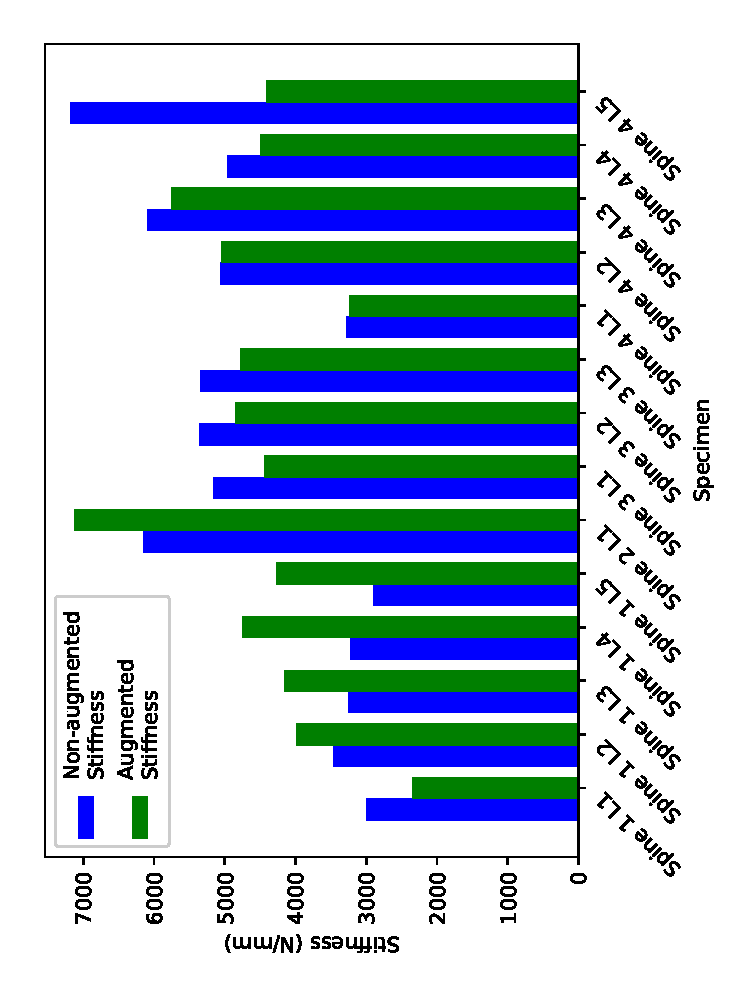
\includegraphics[width=.7\textwidth,angle=270]{Chapters/Chapter_HT_images/aug_non_aug_stiffness}
	\caption{The experimental stiffness of the vertebrae pre and post
augmentation. Showing that 5 of the 14 vertebrae showed an increase in
stiffness following augmentation.}
  \label{fig:aug_non_aug_stiffness}
\end{figure}

A strong relationship was found between the percentage fill volume achieved and the
bone volume fraction of the vertebra, where a reduced density of bone resulted
in larger quantities of cement being injected into the vertebra before cement
leakage occurred.
This relationship can be seen in \cref{fig:cmt_fill_vs_bvtv}.

\begin{figure}[ht!]
  \centering
 
\includegraphics[width=.7\textwidth]{Chapters/Chapter_HT_images/cmt_fill_vs_bvtv.png}
	\caption{The relationship between the percentage cement fill of the total
vertebral volume  achieved through the augmentation procedure and the bone
volume fraction value for each vertebra. }
  \label{fig:cmt_fill_vs_bvtv}
\end{figure}

There was not a clear relationship found between the cement fill of the total
vertebral volume and the resulting change in stiffness following augmentation
for the set of vertebrae on the whole.
However, trends could be seen when splitting vertebrae into groups with:
\textit{a)} dispersed volumes of injected cement and \textit{b)} concentrated
volumes of cement.
This can be seen in \cref{fig:aug_cmt_fill_vs_ch_stiff} where a trend
($r=0.83$) can be seen between the percentage fill of the total vertebral
volume and the percentage change in stiffness for those vertebrae with
concentrated volumes of cement.

\begin{figure}[ht!]
  \centering
 
\includegraphics[width=.7\textwidth]{Chapters/Chapter_HT_images/Aug_cmt_fill_vs_ch_stiff.png}
	\caption{The relationship between the percentage fill of the total vertebral
volume and the percentage change in the vertebral stiffness following
augmentation. The line and \textit{r} value are for the red points where the
cement volume was characterised as concentrated. The remaining blue points
indicated the vertebra where the cement volume was characterised as
dispersed.}
  \label{fig:aug_cmt_fill_vs_ch_stiff}
\end{figure}


The cement distributions following augmentation can be seen in \cref{fig:Spine
1_projection,fig:Spine 2_projection,fig:Spine 3_projection,fig:Spine
4_projection}.
From the 3D projection images and slices from $\mu$CT stack it was determined
which vertebrae contained dispersed and which vertebrae contained concentrated
volumes of cement, this characterisation can be seen in \cref{tab:conc_disp}.



\begin{figure}[ph!]
 \centering
 
\includegraphics[width=.65\textwidth]{Chapters/Chapter_HT_images/G17-11_projections}
	\caption{Transverse and sagittal 3D projection views of the Spine 1 spine
following augmentation, with the cement region being the brighter material in
the vertebral body. The L1 vertebra is defined as having a dispersed volume of
cement while the remaining L2, L3, L4, L5 vertebrae have concentrated volumes
of cement.}
  \label{fig:Spine 1_projection}
\end{figure}

\begin{figure}[h!]
  \centering
 
\includegraphics[width=.65\textwidth]{Chapters/Chapter_HT_images/G19-11_projections}
	\caption{Transverse and sagittal 3D projection views of the Spine 2 spine
following augmentation, with the cement region being the brighter material in
the vertebral body. The vertebra is defined as having a dispersed volume of
cement.}
  \label{fig:Spine 2_projection}
\end{figure}

\begin{figure}[h!]
  \centering
 
\includegraphics[width=.65\textwidth]{Chapters/Chapter_HT_images/G21-11_projections}
	\caption{Transverse and sagittal 3D projection views of the Spine 3 spine
following augmentation, with the cement region being the brighter material in
the vertebral body. The L1 vertebra is defined as having a dispersed volume of
cement while the remaining L2 and L3 vertebrae have concentrated volumes of
cement.}
  \label{fig:Spine 3_projection}
\end{figure}

\begin{figure}[ph!]
  \centering
 
\includegraphics[width=.65\textwidth]{Chapters/Chapter_HT_images/G41-11_projections}
	\caption{Transverse and sagittal 3D projection views of the Spine 4 spine
following augmentation, with the cement region being the brighter material in
the vertebral body. The L1, L2 and L5 vertebrae are defined as having a
dispersed volume of cement while the remaining L3 and L4 vertebrae have
concentrated volumes of cement.}
  \label{fig:Spine 4_projection}
\end{figure}


\begin{table}[h!]
	\caption{The characterisation of the augmented vertebrae into vertebrae with
dispersed and concentrated volumes of cement.}
	\label{tab:conc_disp}
	\centering
	\begin{tabular}{c|c}
    Vertebra & Cement Distribution \\
    \hline
    \hline

    Spine 1 L1 & Dispersed \\
    Spine 1 L2 & Concentrated\\
    Spine 1 L3 & Concentrated\\
    Spine 1 L4 & Concentrated\\
    Spine 1 L5 & Concentrated\\
    Spine 2 L1 & Dispersed \\
    Spine 3 L1 & Dispersed \\
    Spine 3 L2 & Concentrated\\
    Spine 3 L3 & Concentrated\\
    Spine 4 L1 & Dispersed \\
    Spine 4 L2 & Dispersed \\
    Spine 4 L3 & Concentrated\\
    Spine 4 L4 & Concentrated\\
    Spine 4 L5 & Dispersed \\
    \hline
	\end{tabular}
\end{table}



\subsection{Computational Results}


\subsubsection{Non-augmented Model Results}

The results of modelling the non-augmented vertebrae can be seen in
\cref{fig:intact_norm_bvtv}, comparing the initial normal method (the method
used with the bovine tail vertebra in the previous chapter) with the best case
using the bone volume fraction method and the results of the sensitivity test
described previously.
The results show a large improvement using the results of the sensitivity tests
and the bone volume fraction method, with a concordance correlation coefficient
improving from 0.55 to 0.86.

The effect of using the bone volume fraction method on the greyscale background
and colour map of the bone density can be seen in \cref{fig:compX4}, where the
much more clearly defined cortical shell and trabecular structure is evident.

The varying greyscale distribution and differences between the different spines
can be seen in \cref{fig:HT_gs_map}. The general trends match the overall bone
volume fraction values described earlier in \cref{tab:bv_tv_anis}, where the
vertebrae from spine 1 show much lower bone volume fractions which matches the
much more blue heat maps when compared to the denser spine 2, 3 and 4. 

\begin{figure}[h!]
  \centering
  \includegraphics[width=.65\textwidth,angle=270]{Chapters/Chapter_HT_images/intact_norm_bvtv}
	\caption{The results of using the normal method and the bone volume
	fraction method to model non-augmented human lumbar vertebrae. Red
shows the agreement using the normal method and blue shows the agreement using
the bone volume fraction method, with the orange dotted line showing perfect
agreement.}
	\label{fig:intact_norm_bvtv}
\end{figure}


\begin{figure}[h!]
  \centering
\includegraphics[width=.65\textwidth]{Chapters/Chapter_HT_images/compX4MethodAvsB.png}
\caption{A and B: The resultant 1 mm$^3$ greyscale background from the normal
and bone volume fraction method respectively, where the brightness in A has
been increased for visibility. C and D: a heat map of the greyscale values
through the mid slice of models from the normal and bone volume fraction method
respectively.}
	\label{fig:compX4}
\end{figure}

\begin{figure}[h!]
  \centering
\includegraphics[width=\textwidth]{Chapters/Chapter_HT_images/HT_gs_map.png}
\caption{The variation in the greyscale distribution across the mid-slice of
the vertebrae from spine 1, 2, 3 and 4. The general density changes as well as
shifting density distributions are visible.}
	\label{fig:HT_gs_map}
\end{figure}
\subsubsection{Augmented Model Results}\label{sec:augcompres}

The optimum results using the image registration and outcomes of the
sensitivity tests, including the explicitly defined needle tracks can be seen
in \cref{fig:aug_init_vs_best} with the green triangles.  This registration
method with the defined needle tracks achieved a CCC = 0.62, the registration
method not using the needle tracks achieved a CCC = 0.46, while the initial
method used (similar to the method used with the bovine tail vertebrae)
achieved a CCC of 0.18. Comparing the method using the registration method to
the method using the registration method with defined needle tracks,
computationally stiffer vertebrae were weakened and computationally weaker
vertebrae were stiffened due to the higher Young's modulus for the interface
and cement regions.

\begin{figure}[h!]
  \centering
	\includegraphics[width=\textwidth]{Chapters/Chapter_HT_images/aug_init_vs_best_vs_ndl_trcks}
	\caption{The results of using the initial method (red circles), the
registration method (blue triangles) and using the defined needle tracks (green
triangles), showing the agreement to the perfect x=y line in orange.}
	\label{fig:aug_init_vs_best}
\end{figure}


\section{Discussion}

The outcomes of this human vertebrae study are discussed in the following
subsection. Split into three, discussing the experimental results, limitations
and finally the results of the computational aspects of the study.

\subsection{Experimental Results} \label{sec:exp_disc}

Experimentally there was large variation seen in the results, in terms of
material properties (BV/TV values), geometry and response to loading.  The
experimental response to loading showed a large range in the stiffness values
of the vertebrae, even for vertebrae with similar volumes and for vertebrae
originating from the same spine.  This wide range of stiffness' extends to the
augmented vertebral stiffness, although the range does decrease following
augmentation.  The variation seen in the intact vertebrae aids the
justification for the study, if such a wide range of vertebral properties
exists within such a small data set then it explains why such variation is
found clinically when identifying the response to vertebroplasty. For example
in the some of the randomised clinical trials were no statistical significance
in the output measures could be found and in studies of the epidemiology of vertebral fractures
\cite{Buchbinder2009a,Kallmes2009,MeltonIII2006}.
Some of the variation in the stiffness of the non-augmented
vertebrae may be due to the different curvatures in the spines of people. These
different curvatures will lead to different loads through the same vertebral
level in different people and may explain why little differentiation between
spinal level can be made. The different loading regime at the same level means
that the density distribution within the vertebrae varies and hence to optimum
location for the injected cement volumes would also vary. This idea of spinal
level, varying loads and vertebral density is explored further in
\cref{sec:lpe}.

Following augmentation five of the 14 vertebrae showed an increase in the
stiffness, which, given the stiffness of the injected cement compared to that
of trabecular bone, is an unexpectedly small number. However, this is not
entirely unexpected, with a similar range of increases and reductions seen in
the study by Wijayathunga et al. \cite{Wijayathunga2008} and no statistical
difference in the studies by Kinzl et al.
\cite{Kinzl2012,kinzl2013experimentally,Kinzl2012a} unless the cement
distribution was distributed to both of the endplates, forming a column of
cement from the superior to the inferior.
Four of the vertebrae that showed an increase in stiffness were
from the same spine (Spine 1), which is the spine that had a considerably
smaller bone volume fraction compared to the other vertebra from other spines.
Given that this spine had the smallest bone volume fraction it also received
the largest quantity of cement, given the relationship between the percentage
fill achieved and the bone volume fraction.  This relationship is most likely
due to the ease of cement injection before leakage, with more dense vertebrae
failing to receive large volumes of cement before the cement found one of the
vascular channels (upon which injection was stopped) and less dense vertebrae
having more space to receive cement. So, the reduced BV/TV and therefore
density of Spine 1 allowed both larger volumes of cement to be injected and due
to its reduced density was more receptive to having its stiffness increased
through augmentation. This may suggest that these type of vertebrae are the
best candidates for the procedure given the risks of damage through the high
intra-vertebral pressures that can be generated
\cite{aquarius2014prophylactic,gravius2009intravertebral}. In cases where the
vertebral density is high, but high fill volumes are still pursued damage may
be caused by the high pressures ``pushing" trabeculae to the side.
Interestingly and converse to findings presented here, the study by Aquarius et
al. \cite{aquarius2014prophylactic} suggested that cement volumes like those
described here as concentrated were caused by high pressures ``pushing"
and damaging trabeculae. The more dispersed distributions gave more
interdigitation due to the lower pressures and therefore resulted in reduced
damage and stiffer augmented vertebrae. However, it may be the case that these
dispersed and concentrated volumes described here are a different phenomenon to
the ball shaped and irregular shaped cement distributions described in that
study. A potentially worrying consequence of the high pressures during the
injection is the filter pressing that can occur
\cite{tarsuslugil2013development}, here, separation of the radio-opacifier from
the cement is possible, meaning that experimentally and clinically (through
fluoroscopy) the extent of the injected cement volume is potentially unknown.
Additionally from a modelling perspective, a potential separation of the liquid
and powder components of the PMMA may result in changing material properties of
the cement region.

Cement volume positions were generally to the anterior of the vertebrae and to
the middle of the inferior-superior plane, matching the desired position
\cite{Nice2013}
achieved through the insertion of the needle and angling of the side opening
needle tip. 
Given the lack of obvious
variation in cement positions and shapes it was difficult to characterise the
cement distributions, hence, a simplified description of the cement was used.
This simplified description of the cement described whether the cement was in a
concentrated volume or dispersed in a larger region or whole vertebra.
Following this
characterisation strong relationships were found between the change in
stiffness and percentage fill, if only those vertebrae with a concentrated
volume of cement were included.  Suggesting that distributed volumes of cement
are difficult to predict and should be avoided when carrying out the procedure
using fluoroscopy, especially with more dense vertebrae where the likelihood or
disperse volumes of cement increased.
Many previous studies only found significant increases in the stiffness of
augmented vertebrae when the cement distribution was endplate to endplate
stretching from the superior to the inferior of the vertebral body
\cite{Chevalier2008,aquarius2014prophylactic,steens2007influence}. The sagittal
views of the augmented vertebral projections suggest that all vertebrae except
Spine 2 L1 and Spine 3 L1 achieved such end-to-end distributions with no
noticeable difference in the change in stiffness of these two vertebrae,
especially given that the Spine 2 L1 vertebrae received a large increase in
stiffness following vertebroplasty..

To summarise the change in stiffness following augmentation based on the
material properties of the vertebrae, the following features have the greatest
effect: 
\begin{enumerate} 
	\item A smaller bone volume fraction results in
	larger quantities of cement being injected before leakage occurs.
	\item If the volume of cement is contained in a concentrated volume then the
	greater the volume of cement then the larger the increase in stiffness
	following augmentation.  
	\item If the volume of cement is dispersed
	through the vertebral body then there is no relationship between the
	volume of cement injected and its effect of the vertebral stiffness.
	\item Concentrated volumes of cement are more likely if the bone volume
	fraction of the vertebra is lower (and therefore has a reduced density).
\end{enumerate}

The effects of vertebral geometry and material properties on the response to
augmentation will be investigated further using statistical shape modelling in
\cref{PCA_CHAP}, giving a more detailed story of the suggested approaches to
vertebroplasty based on the tests carried out in this study.

\subsection{Limitations Regarding Specimen Numbers \& Vertebral Features}

One of the main limitations to the study is the numbers of vertebrae included
in in the set.  Having four human spines with a limited number of lumbar
vertebrae available from each spine, meant that only 14 out of a possible 20
vertebrae were able to be tested.  This meant that there was a skew towards the
top of the lumbar section with limited numbers of L4 and L5 vertebrae.  Such
skews to the data set have effects to any statistics applied to the data set
and will be discussed more thoroughly in the chapter on Statistical Shape and
Appearance modelling, \cref{pca_disc}.  More relevant to modelling the
vertebrae is the effect this has on the determination and optimisation of the
greyscale conversion factor.  The large change in geometry from L4 to L5,
rather that the gradual change between L1 to L4, introduces questions about the
response to loading (and augmentation) for this vertebra in particular and how
it differs from other levels.  A resolution to this limitation would be to
increase the specimen numbers and look at vertebral levels in isolation;
identifying level specific differences and properties.  Variation at different
vertebral levels may require level specific greyscale conversion factors, such
as those required when modelling different animal species
\cite{zapata2017methodology}.  However, within the current set of vertebrae
greater variation was found between spine rather than level (for BV/TV,
stiffness and vertebral body volume), even when including L5 vertebrae.
Suggesting that segregation of vertebral levels is unnecessary for the current
specimen set. %TODO MAYBE talk about the effect of vb leve, curvature, density AGAIN, DO NOT REPEAT THE ABOVE!!!!

Another limitation of the study is the age range and limited information
regarding vertebral health.  Because of the unknown vertebral quality or health
it was decided to skip the initial load to failure carried out in the bovine
tail study.  While no evidence of fractures could be seen in the $\mu$CT scans,
other than slight wedge shapes, there was also no evidence of the bovine tail
vertebrae having succumbed to fracture in $\mu$CT either, despite clear
fractures on load displacement curves.  Therefore the state of the vertebrae
was relatively unknown in their pre-augmented state and the study therefore
becomes an investigation into the effects of prophylactic vertebroplasty
similar to a number of previous studies
\cite{higgins2003biomechanical,furtado2007biomechanical,oakland2009preliminary},
although with the possibility that some of the vertebrae were fractured
\textit{in vivo}. 


\subsection{Computational Results}

Many developments in the computational methods have been made through the
course of this chapter, with the resulting improvements showing their
importance. The significance of these developments and the results is discussed
in the following subsections, split into a discussion of the improvements to
modelling non-augmented vertebrae, augmented vertebrae and the results of
various sensitivity studies.


\subsubsection{Non-augmented Models}

The improvement in the agreement between computational stiffness and the
experimental stiffness results using the bone volume fraction method and the
results of the sensitivity tests is significant and provides a good foundation
for modelling the more challenging augmented models. The improvement using the
bone volume fraction method in isolation (without the results of the other
sensitivity tests) showed a large improvement over the normal method.  The
normal method performed similarly on the bovine tail vertebrae as with the
human lumbar vertebrae, with a CCC = 0.49 for bovine tail vertebrae and CCC =
0.55 for the human vertebrae. 

The small improved agreement of modelling the human vertebrae over the bovine
vertebrae when using the same ``normal" method suggests that either the human
vertebrae are more receptive to the modelling method used, or that the
experimental procedure was more repeatable and therefore provided more accurate
results. One possibility is that the less narrow human vertebrae provided an
easier material to load axially, with slight off axis loads causing the
vertebrae to not be seated in the endcaps correctly in the case of the bovine
tail vertebrae. This sensitivity to endcap contact properties was shown earlier
and given the tendency of the bovine vertebrae to be loaded non-axially (due to
their narrow columnar shape) they may be more sensitive to such endcap contact
properties. So, while experimentally the bovine vertebrae were able to slip in
the endcaps, computationally the two materials were tied, restricting this
ability and reducing the agreement with the experiment. Conversely, the wider
human vertebrae had less of a tendency to slip and were less sensitive to the
endcap contact. This change to the endcap contacts seems to be a common
transition from similar studies where tied contacts were used
\cite{Wijayathunga2008} to more recent studies
\cite{kinzl2013experimentally,Kinzl2012a}, however the property is rarely
presented in the literature.

The improvement using the bone volume fraction method is most likely due to the
added definition of the trabecular bone and cortical shell, especially given
how important the correct representation of load sharing is for accurate models
\cite{eswaran2006cortical}. This agreement is much stronger than the agreement
found in similar studies that used a comparable methodology to the ``normal"
method \cite{Wijayathunga2008, zapata2017methodology, RobsonBrown2014} and
comparable to methods that used more complex although individual material
properties for each model \cite{Kinzl2012,kinzl2013experimentally}. An
advantage the current study has over these latter studies is a uniform material
property that once calibrated over a large set of vertebrae can be used on any
unseen human lumbar vertebrae. Having greater definition of the cortical shell
and trabecular bone alignment allows much more accurate descriptions of the
load transfer through the vertebrae, rather than the more simple description
with the more homogenised material properties of the normal method.

This method also removed any effect that the bone marrow, where, given the
freeze/thaw cycles the marrow leaks from the vertebrae giving vertebral scans
with portions of the bone marrow missing and therefore changing the greyscale
background and material properties.  Due to the initial segmentation and
binarisation at 82 $\mu$m using the BV/TV method the bone marrow is not present
in the segmented full resolution or downsampled scans and therefore has no
impact on the material properties of the models.  Conversely, using the normal
method, areas lacking bone marrow would have a lower Young's modulus and areas
with bone marrow would have higher Young's moduli, not corresponding to the
actual properties of these regions and changing the load distribution.

One of the limitations of the bone volume fraction method is that is relies on
having trabecular resolution scans of the vertebrae to apply the trabecular
bone thresholds to. 
This is a similar limitation to studies that also achieved a good agreement
between computational and experimental results of augmented stiffness
\cite{kinzl2013experimentally}, where high resolution $\mu$CT scans were
required for the acquisition of BV/TV and fabric information for their
methodology.
This limits the origin of the scans to \textit{in vitro}
scans rather than \textit{in vivo} scans where the standard clinical resolution
is limited to approximately 1 mm and larger.  Given the intention to generate
larger populations of vertebra models for use in statistical shape modelling
this limit to scan origin is an unwanted consequence.  A possible solution to
this problem would be to use 16 bit images rather than the currently used 8 bit
images.  This change gives an increase in the number of greyscale values
available from the 256 of 8-bit images to over 65,000 for 16-bit images.  The
main benefit of the bone volume fraction method is the increased definition of
bone structure and a greater contrast between the brighter, denser cortical
bone, the trabecular bone and the empty, non-bone areas.  Using 16-bit images
along with image manipulation to change the contrast of the scans may allow the
added detail and contrast to be captured with relatively low ($\geq$ 1 mm)
resolution scans, therefore greatly increasing the number of vertebral
specimens available for use. An example of how this could be achieved is shown
in \cref{fig:adding_contrast} where the background from the normal method has
been edited through adjusting the contrast to give a similar background to that
achieved using the bone volume fraction method. The detail in the centre of the
vertebral body is less clear in this example, however, it was achieved through
simple contrast manipulation of the 8 bit TIFF stack, meaning that more
trabecular detail could be preserved using a curves (remapping of the image
tonality) and/or as already proposed, 16 bit images.

\begin{figure}[h!] \centering
	\includegraphics[width=.65\textwidth]{Chapters/Chapter_HT_images/adding_contrast.png}
	\caption{An example showing the ability to create a greyscale
		background similar to that achieved using the BV/TV method, but
		instead adjusting the contrast of the background from the
normal method.} \label{fig:adding_contrast} \end{figure}

\subsubsection{Augmented Models}

The results of modelling augmented vertebrae showed a reduction in the
agreement when compared to the non-augmented vertebral models, mirroring that
found by Wijayathunga et al. \cite{Wijayathunga2008}.
Reasons for this are centred
around modelling the internal cement region, given the good agreement seen
between the non-augmented vertebrae and their models.  More specifically the
problems in modelling the cement region may be due to experimental and
modelling techniques.  

Issues originating from the experimental work come from the difficulty in
capturing the extent of the injected cement volume, often due to clumping of
the barium sulphate and separation of the barium sulphate from the other
components of the PMMA cement.  The clumping of barium sulphate was also found
by Sikora \cite{Sikora2013a}, in this study agglomeration was reduced through
vigorous mixing of the PMMA monomer and barium sulphate prior to mixing with
the PMMA powder. However, others suggested that the separation of the barium
sulphate from the cement (calcium phosphate in that study
\cite{tarsuslugil2013development}) during the high pressures of the injection
were the cause of the subsequent agglomeration.  While this problem is
minimised through segmentation of the cement region at higher resolutions
before the downsampling, a problem still lies in capturing the intricate
interdigitation between the cement and the trabecular bone at a resolution of 1
mm.  One issue overcome through the use of the registration method is the
removal of the bright halo of the cement region (from clumps of barium
sulphate) solving the problems found in the previous chapter using bovine tail
vertebrae and problems encountered by others \cite{Wijayathunga2008,Sikora2013a}.
This allowed more accurate modelling of the material
properties of the vertebral bone and additionally better accuracy of modelling
the interface, given the removal of the false, dense bone surrounding the
yielding interface in the bovine tail models. The inclusion of the explicitly
modelled needle tracks increased the agreement significantly, with the
compromise of interrupting an otherwise automated modelling process.

An additional experimental challenge is the unknown level of damage caused to
the vertebrae when the needle is inserted.  Given that after clear fractures
(based on load-displacement curves), damage could not be seen on 82 $\mu$m
scans of bovine tail vertebrae, it is unlikely that micro-fractures caused
through needle insertion will be captured in the $\mu$CT scans of the human
vertebrae. Further tests could investigate whether a change to the Young's
modulus as a function of the density in the areas surrounding the needle tracks
would improve the agreement. This could represent either damage to the bone in
the form of micro-fractures or the compacted bone created by the needle.

Despite the reduced agreement of the augmented models, there was a large
improvement compared to the initial method, which was the method used for
modelling augmentation in the bovine tail vertebrae.  As with the non-augmented
models the CCC using the initial method was very similar to the CCC using the
comparable method on the bovine tail vertebrae, CCC = 0.18 and 0.15 for the
human and bovine models respectively.  This makes the improvement using the
registration significant and a beneficial step in making the models of
augmented vertebrae.

Achieving improved agreement between the computation and experimental models is
an obvious next step for the project and despite the range of approaches used
to improve the agreement, there are some next steps.  Given the difficulty
capturing the detail between the cement and trabecular bone, using a higher
resolution is a clear next step.  However, it comes with a number of
difficulties which have been shown in the study by Zhao et al. \cite{Zhao2012},
where the increase in resolution presents many other unknowns that need to be
modelled.  For example modelling the specific interaction between the bone and
the cement including the  coefficient of friction between them.  This would
require difficult experimental investigations, given the unique environment
inside the vertebrae filled with bone marrow.  Along with modelling properties
that are not applicable in continuum level models, there is the problem with
computational cost, where the increased time to solve models would become
problematic given the investigatory nature of the study and the fact that the
behaviour in simplified bone plug models is different to what is seen in whole
vertebrae \cite{Sikora2013}. Perhaps the methods used by Kinzl et al.
\cite{kinzl2013experimentally} would form a middle ground between the two
approaches. In that study, spheres were randomly inserted into the
augmentation region to represent the pores that are present, although not
visible in the augmented regions of the experimentally augmented specimens.
This methodology is similar to one of the approaches attempted in the current
study which unfortunately performed less favourably that the currently
presented approach. It involved an inverse greyscale material property for the
augmented region based on the underlying non-augmented background, where empty
(marrow containing) voxels were given material properties of, or close to PMMA,
voxels that contained trabecular bone were given the material properties of
bone and intermediate greyscale values attempted to represent the gaps that
form as the cement shrinks during setting. This methodology and preliminary
results can be seen in \cref{sec:invGS}.

\subsubsection{Sensitivity Test Significance and Influence on
Errors}\label{sec:errors}

Sources of error from modelling come from discrepancies between the
experimental setup and specimen geometry and material properties. Sensitivity tests carried out
identified the effect of errors in accurately describing the cement cap depth
and loading position accuracy, given the 1~mm accuracy limit. The maximum
possible error for load position in a $\pm$1~mm anterior/posterior/left/right
direction was less than 5\%, with the worst case error for the for the encap
depth tests (1~mm thicker for both endcaps) being approximately 5\%. Other
possible errors would include accurately capturing the model geometry, however
simply eroding or dilating the vertebral mesh would not accurately describe the
type of meshing errors that may occur (it is unlikely that masks would be
created at $\pm$ 1 voxel around the whole model). To attempt to answer this a
user variability test was carried out in \cref{sec:uvs}. There, the maximum
user variability gave errors of 14 \%, however as discussed in that chapter,
users achieved consistently higher or lower stiffness' compared to their peers.
Hence, a 14 \% error within a single users segmentation process is both
unlikely and further reduced through the use of the python script carrying out
the thresholding and morphological filters to segment the model.  Therefore
simply adding the two main sources of error gives a worst case error of
approximately 10 \%, an error which when compared to the possible errors in
obtaining the maximum stiffness and the errors between loading repeats, is
negligible. The specific error in the experimental load is difficult to measure
mainly due to the high value and limited supply of human tissue; to measure the
error in repeated loads more accurately, these repeats would need to be
taken in the non-augmented state given the large array of unknowns the
augmentation process introduces. However, this would have led to possible
damage or unwanted fracture of the vertebrae, making the results following
augmentation more difficult to interpret. As it stands the differences between
repeats of the augmented vertebrae show changes of approximately -3000 N/mm to
+1200 N/mm, with the large reductions originating from  repeated testing in plastic regions
of the load displacement curve. These large errors between repeated measures
are the worst case however and it is unlikely that such errors would occur
between non-augmented specimens in a loading range that avoids the potential of
causing damage. Suggesting that the results presented here, being the
consequence of 2 loads total (one non-augmented, one augmented), have much less
error than that seen in the repeated loads.

In addition to error in measuring the stiffness, errors in the measurement of
the maximum stiffness also exist due to the cut off at 1600 N in the
experimental loading. This meant that for some of the vertebrae the maximum
stiffness was not reached and therefore not captured in the load displacement
curve. A prediction of the failure stress and an estimation of the failure
load through simulation of a vertebra prior to experimental loading
could help to remove this problem. However, this would have required yet
another set of human vertebrae.

Changing the endcap depth presents an interesting study into the effects of
over constraining the models. For the models with the tied constraints changing
the endcap depth had a different effect for the two vertebrae (although the
same overall trend, where thicker endcaps led to more constraint and therefore
higher stiffness values). The spine 1 L2 vertebrae was equally sensitive to
changing the superior and inferior depth, although gave a smaller effect when
the depth was reduced (exposing more bone). The spine 4 L5 vertebrae was much
more sensitive to changing the inferior endcap, especially when reducing the
depth of the endcap. This large reduction in the stiffness, when removing 3 mm
of endcap material from the inferior endcap, of approximately 20 \% is caused
by exposing a less dense area of bone, which, when no longer supported by the
tied endcap resulted in the reduced stiffness. Other than this specific effect
the general trend was an increased sensitivity to increasing the cement depth,
with a much smaller sensitivity to exposing more bone.

Changing the endcap depths when the frictionless contact was used resulted in
(for the most part) much less sensitivity to changing the endcap depth, when
compared to the tied endcap models. The exception is the spine 4 L5 vertebra,
where when the endcap depth is reduced a very large decrease in the stiffness
is seen. This is caused by slipping that occurs between the vertebrae and the
endcap, given the lack of both physical constraint and constraint in the form
of a boundary condition. An illustration of this can be seen in
\cref{fig:EC-3slip}, showing that with such little constraint the anterior
inferior of the vertebral body moves further to the right (anterior). This
results in the reduced stiffness recorded. However, such small endcaps where
not created experimentally and therefore create no additional errors to the
models.  Importantly, the use of frictionless contact with the ``no separation
after contact" option set results in smaller sensitivity to endcap depth
modelling errors and resulted in increased agreement between experiment and
model for the whole set of 14 vertebrae.


\begin{figure}[h!] \centering
	\includegraphics[width=.65\textwidth]{Chapters/Chapter_HT_images/EC-3slip.png}
	\caption{An illustration of the slipping that occurs in Spine 4 L5 when
	the endcap depth is reduced by 3 mm on the superior and inferior
endcaps} \label{fig:EC-3slip} \end{figure}

The effect of changing the loading position aided the understanding of the
mechanics of the models and their response to loading. Experimenting with
different loading positions allows development of our understanding of the
response to different natural loading conditions that would be experienced
during daily life. This could help to answer the important question of how
vertebroplasty effects adjacent level loading and how it may effect the chances
of adjacent level fracture. However, these investigations have been carried out
in \cref{PCA_CHAP} where the response to loading following augmentation was
investigated and, given the more systematic nature of the generated models,
allowed for an easier interpretation of the results. Here, the response to
loading outside of the $\pm$1 mm error range follows a mostly expected pattern
with loads anterior, posterior, left and right at $\geq$ 10 mm away from the
central loading position resulting in progressively reducing stiffness. The
reduced material beneath the axial loading point explains most of these
results, with the greater reduction when loaded anteriorly being due to the
generally reduced density of the anterior portion. The smaller reduction in the
stiffness when loaded posteriorly is due to the increased density which was in
the posterior region of most of the vertebrae, which was seen in the greyscale
density maps of the set. The anomalous result is the Spine 3 L2 vertebra, where
posterior loading of 10 mm behind the central loading position resulted in an
uncharacteristic increase in the measured stiffness.  The Spine 3 L2 vertebrae
had particularly degenerated superior and inferior endplates, protruding
anteriorly at both ends, but with little protrusion posteriorly.  This meant
that when measuring the central loading position experimentally, a loading
point was selected further anterior than what would have been picked without
the bone growths. This explains why moving the loading position further to the
posterior resulted in an increased stiffness with respect to the central
loading point, given that the central loading point was actually placed
anteriorly and hence had a smaller stiffness than expected.  This presents
another reason for why carrying out load position tests on the generated models
in \cref{PCA_CHAP} is preferred, there, central loading can be ensured and the
requirement to match the experimental loading position is removed.


\section{Conclusion}

Overall the models produced here can estimate the stiffness of non-augmented
human lumbar vertebrae to a very high degree. The prediction abilities of
models of vertebroplasty is reduced, although a large improvement over studies
that used similar approaches and had similar constraints in mind (clinical
resolutions for scans etc.). Importantly, the models can represent the large
range of outcomes from the augmentation process, suggesting that the
representation of augmentation is robust enough to model and experiment with
different augmentation scenarios. Therefore providing a good starting point to
use statistical shape and appearance modelling to understand the intricacies of
vertebroplasty.





